\begin{document}

\begin{frame}
\titlepage
\end{frame}

\begin{frame}

\frametitle{PostgreSQL histórico}

 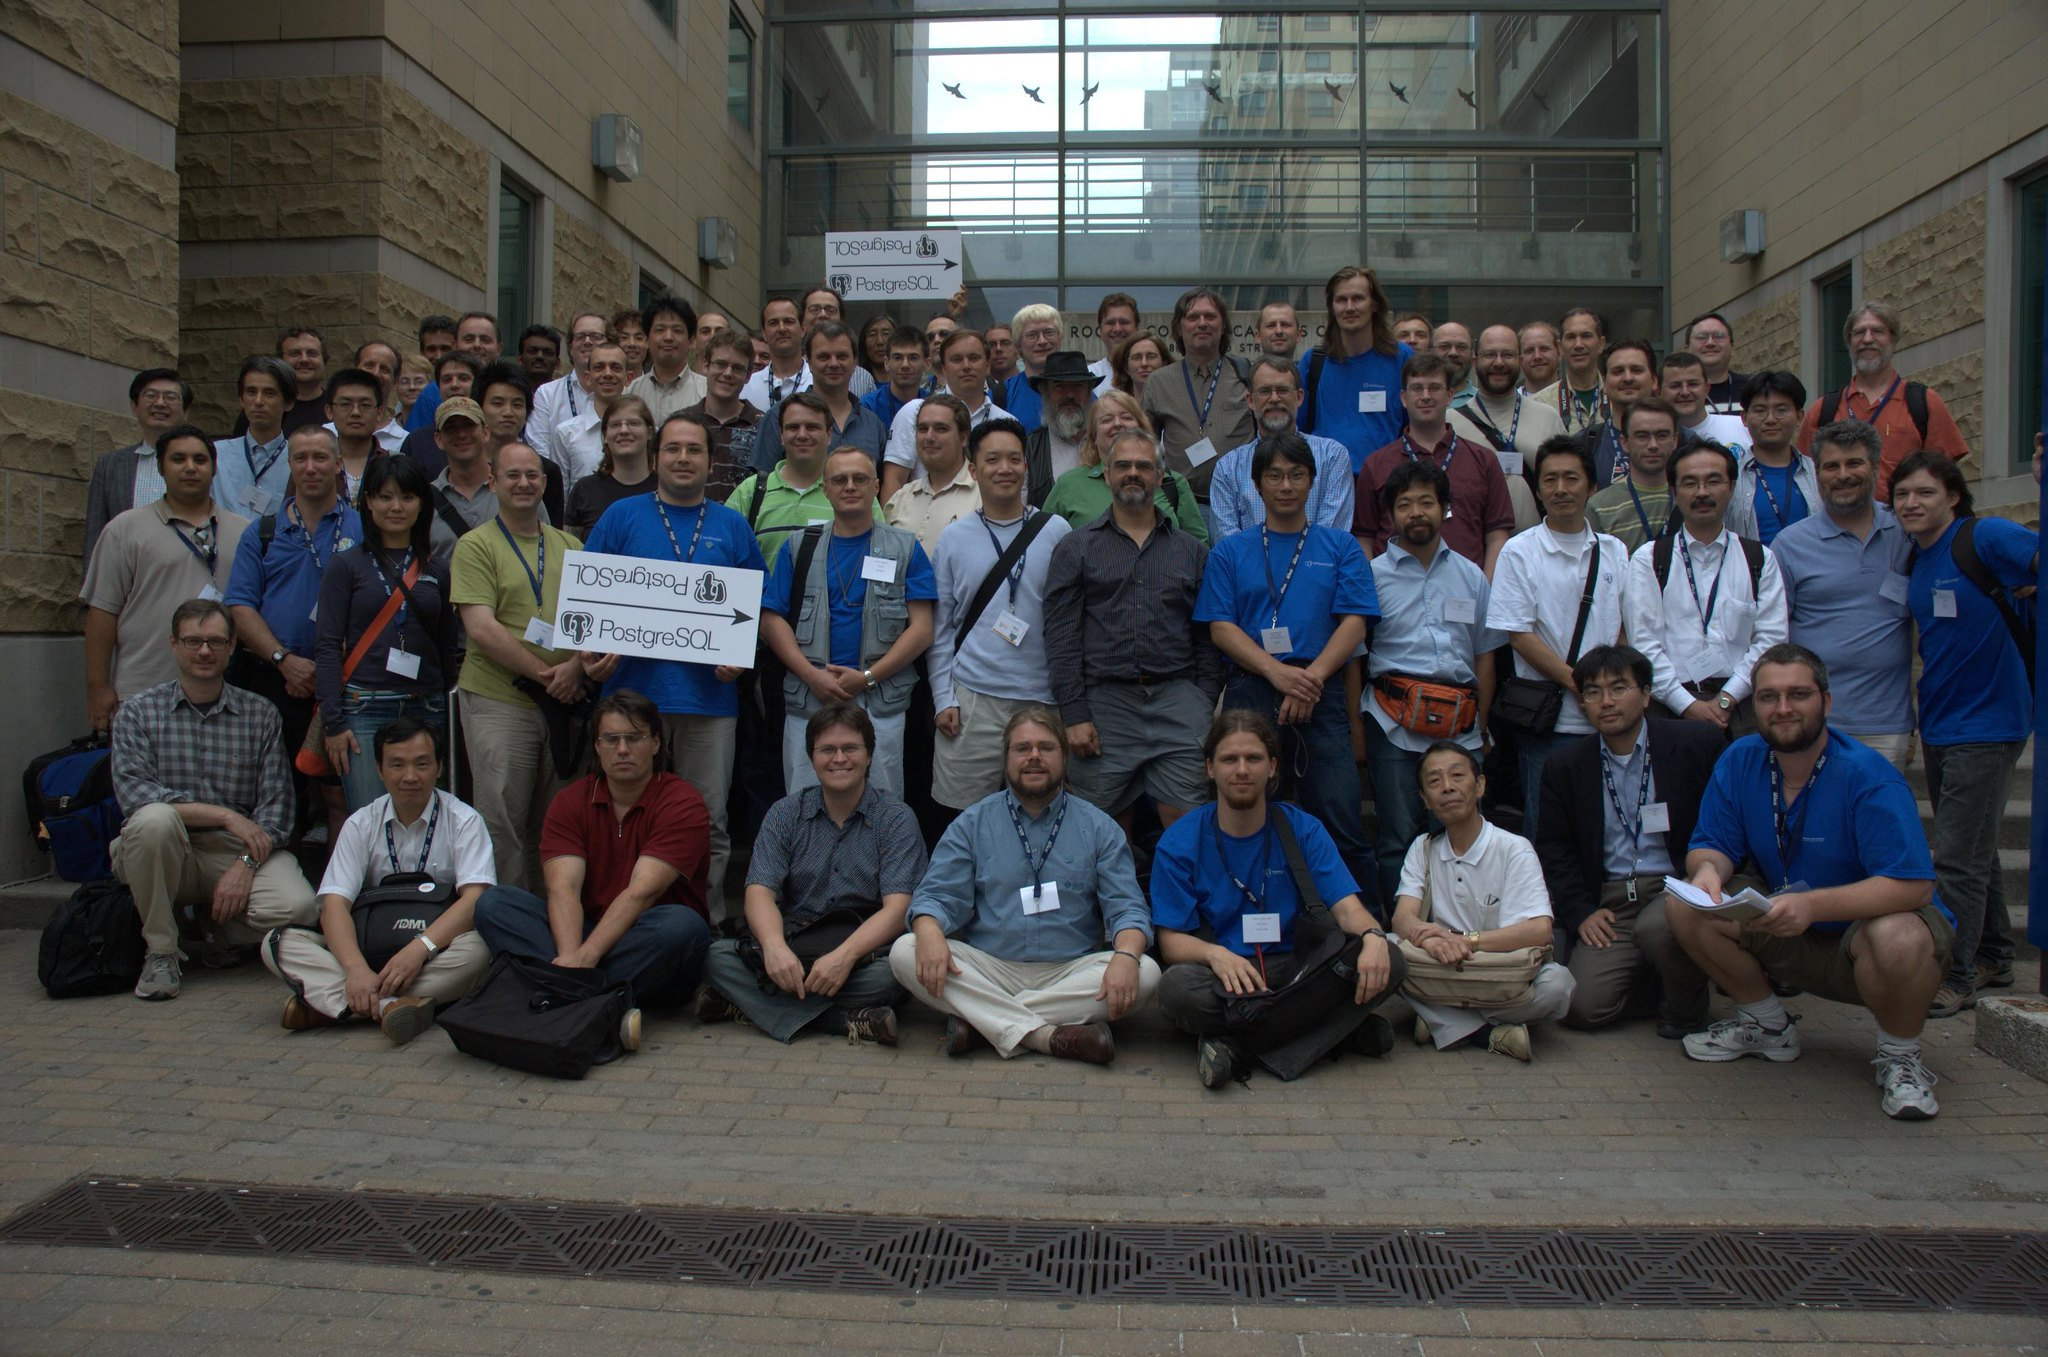
\includegraphics{anniv.jpg}

 \footnotesize
PostgreSQL Anniversary Summit, Toronto, Canadá, 2006

\end{frame}

\begin{frame}

\frametitle{PostgreSQL moderno}

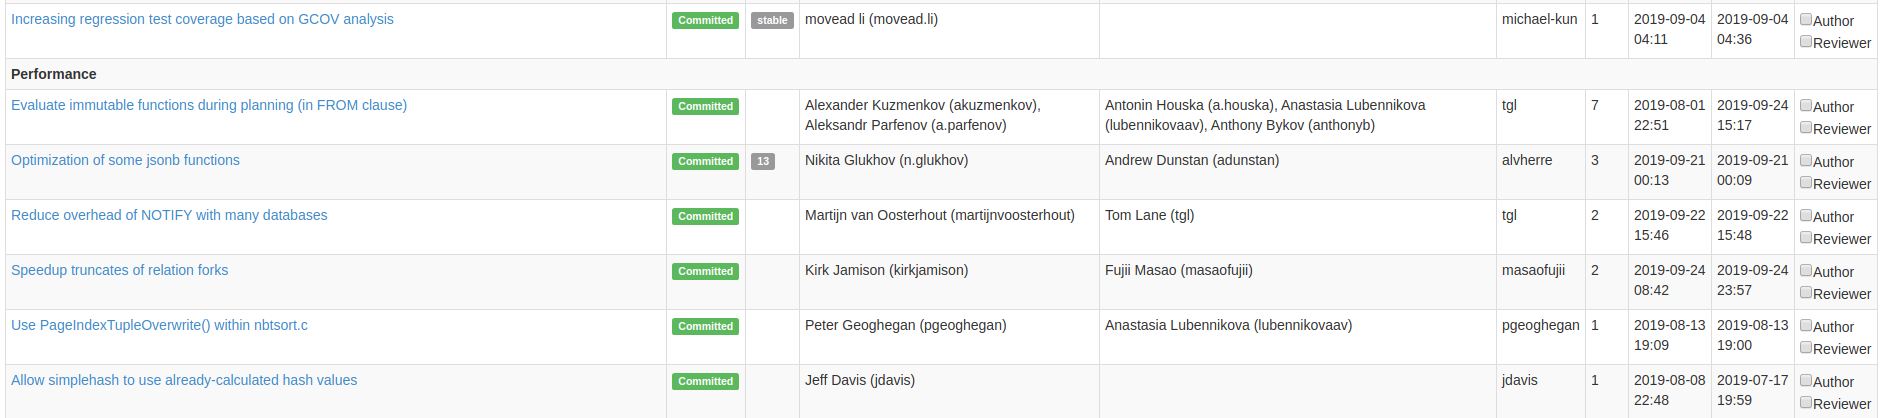
\includegraphics{cfpatches.png}
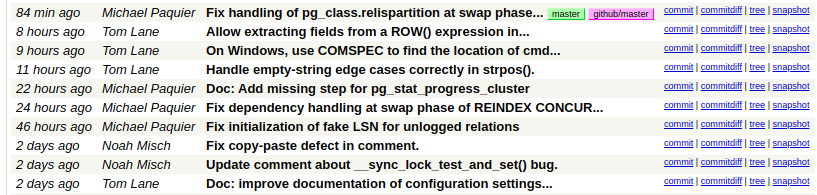
\includegraphics{commits.png}

\hfill \texttt{pgsql-hackers@lists.postgresql.org}

\end{frame}


\begin{frame}
\frametitle{Nuevas bases de datos}

\vfill
\begin{itemize}
\item El término "BD relacional" suena obsoleto
\item Las BDs modernas han avanzado mucho desde SQL:89
\item Cada año,
\begin{itemize}
\item PostgreSQL agrega nuevas tecnologías, nuevos conceptos
\item Se abren nuevos potenciales casos de uso
\end{itemize}
\end{itemize}
\vfill
\end{frame}

\begin{frame}
\frametitle{Líneas de desarrollo}

\begin{itemize}
\item Particionamiento

\item Extensibilidad de almacenamiento
\begin{itemize}
\item zheap
\item zedstore
\end{itemize}

\item Nuevas características del estándar SQL
\begin{itemize}
\item SQL/JSON
\item Temporal query
\end{itemize}

\item \textit{Foreign data}

\item \textit{Sharding}

\item Revolución en el ejecutor
\begin{itemize}
\item JIT
\item ejecución en ``batch''
\end{itemize}

\end{itemize}

\end{frame}

\begin{frame}
\frametitle{Particionamiento}

\begin{itemize}
\item Particionamiento declarativo agregado en PostgreSQL 10
  \begin{itemize}
  \item \texttt{CREATE TABLE PARTITION BY}; estrategias range y list; sin PKs, sin FKs
  \end{itemize}
\item PostgreSQL 11: mucha funcionalidad extra
  \begin{itemize}
  \item Significativas mejoras de rendimiento,  \textit{pruning}
  \item Estrategia \textit{hash}; partición default
  \item DDL adicional: CREATE INDEX; PKs y FKs (con restricciones)
  \end{itemize}
\item PostgreSQL 12: mejoras de rendimiento
  \begin{itemize}
  \item mejor escalabilidad a grandes cantidades de particiones
  \item FKs
  \end{itemize}
\item PostgreSQL 13: mejoras de rendimiento
 \begin{itemize}
 \item mejor \textit{pruning} en \texttt{UPDATE}/\texttt{DELETE}
 \item rehacer parte del optimizador
 \end{itemize}
\end{itemize}
\end{frame}

\begin{frame}
\frametitle{Extensibilidad de almacenamiento}

\begin{itemize}
\item ``table access method''
\item actualmente: \texttt{heapam} $\rightarrow$ VACUUM
\item profundamente ligado al código del servidor
\item Agregar abstracción requirió dos años de trabajo
\item PostgreSQL 12: \texttt{CREATE ACCESS METHOD .. TYPE TABLE}
\end{itemize}

\end{frame}

\begin{frame}
\frametitle{zheap}

\begin{itemize}
\item No+VACUUM
\item basado en \texttt{UNDO}
\item UPDATE/rollback no generan tuplas muertas
\begin{itemize} \item UNDO las limpia \end{itemize}
\item \textit{undo workers}
\end{itemize}

\end{frame}

\begin{frame}
\frametitle{zedstore}

\begin{itemize}
\item A partir de ``table AM''
\item Column stores!
\begin{itemize}
\item Citus: cstore\_fdw
\item Greenplum: AOCO (append-optimized column-oriented)
\item PostgresPro: VOPS
\end{itemize}
\end{itemize}

\footnotesize
\url{https://www.postgresql.eu/events/pgconfeu2019/schedule/session/2738-zedstore-column-store-for-postgresql/}
\end{frame}

\begin{frame}
\frametitle{Nuevas características en estándar SQL}

\begin{itemize}
\item PostgreSQL tiene un miembro en el comité de estandarización!
\end{itemize}
\end{frame}

\begin{frame}[fragile]
\frametitle{SQL/JSON: JSONPATH}

\begin{itemize}
\item PostgreSQL 12: \texttt{JSONPATH}
\end{itemize}
\begin{verbatim}
select * from jsonb_path_query('{"a":[1,2,3,4,5]}',
        '$.a[*] ? (@ >= $min && @ <= $max)',
	'{"min":2,"max":4}');
 jsonb_path_query 
------------------
 2
 3
 4
(3 filas)
\end{verbatim}
\end{frame}

\begin{frame}[fragile]
\frametitle{SQL/JSON: JSON\_TABLE}
\begin{itemize}
\item \texttt{JSON\_TABLE}
\end{itemize}
\footnotesize
\begin{verbatim}
CREATE TEMP TABLE jsonb_table_test (js jsonb);
INSERT INTO jsonb_table_test
VALUES (
   '[
       {"a":  1,  "b": [], "c": []},
       {"a":  2,  "b": [1, 2, 3], "c": [10, null, 20]},
       {"a":  3,  "b": [1, 2], "c": []},
       {"x": "4", "b": [1, 2], "c": 123}
    ]'
);
\end{verbatim}
\end{frame}

\begin{frame}[fragile]
\footnotesize
\frametitle{SQL/JSON: JSON\_TABLE (2)}
\begin{verbatim}
select
   jt.*
from
   jsonb_table_test jtt,
   json_table (
       jtt.js,'strict $[*]' as p
       columns (
           n for ordinality,
           a int path 'lax $.a' default -1 on empty,
           nested path 'strict $.b[*]' as pb columns ( b int path '$' ),
           nested path 'strict $.c[*]' as pc columns ( c int path '$' )
       )
   ) jt;
 n | a  | b | c  
---+----+---+----
 1 |  1 |   |   
 2 |  2 | 1 |   
 2 |  2 | 2 |   
 2 |  2 | 3 |   
 2 |  2 |   | 10
 2 |  2 |   |   
 2 |  2 |   | 20
 3 |  3 | 1 |   
 3 |  3 | 2 |   
 4 | -1 | 1 |   
 4 | -1 | 2 |   
(11 rows)
\end{verbatim}
\end{frame}

\begin{frame}[fragile]
\frametitle{Temporal query}

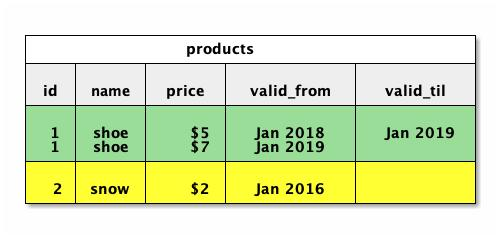
\includegraphics{temporal.jpg}

\begin{verbatim}
ALTER TABLE variants
ADD CONSTRAINT tfk_variants_product_id
FOREIGN KEY (product_id, PERIOD valid_at)
REFERENCES (id, PERIOD valid_at);
\end{verbatim}

\footnotesize\url{https://www.pgcon.org/2019/schedule/events/1336.en.html}

\end{frame}

\begin{frame}
\frametitle{Foreign data \& sharding}

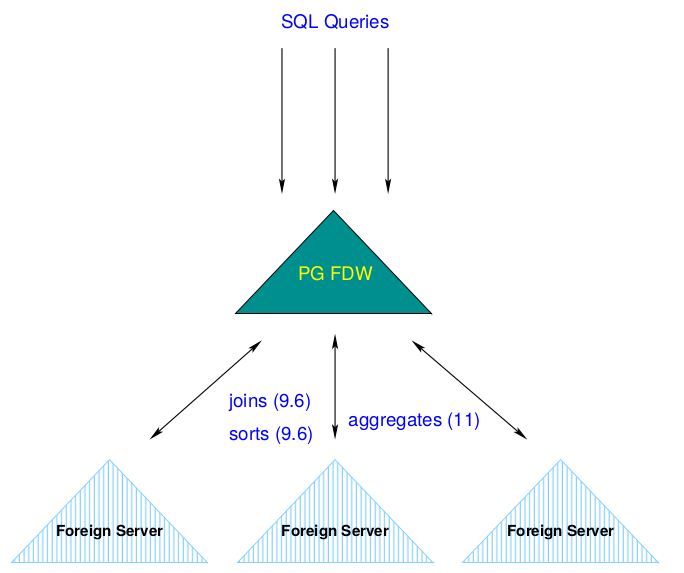
\includegraphics{sharding.png}

\footnotesize\url{https://www.postgresql.eu/events/pgconfeu2019/schedule/session/2581-community-roadmap-to-sharding/}
\end{frame}

\begin{frame}
\frametitle{Foreign data \& sharding (2)}

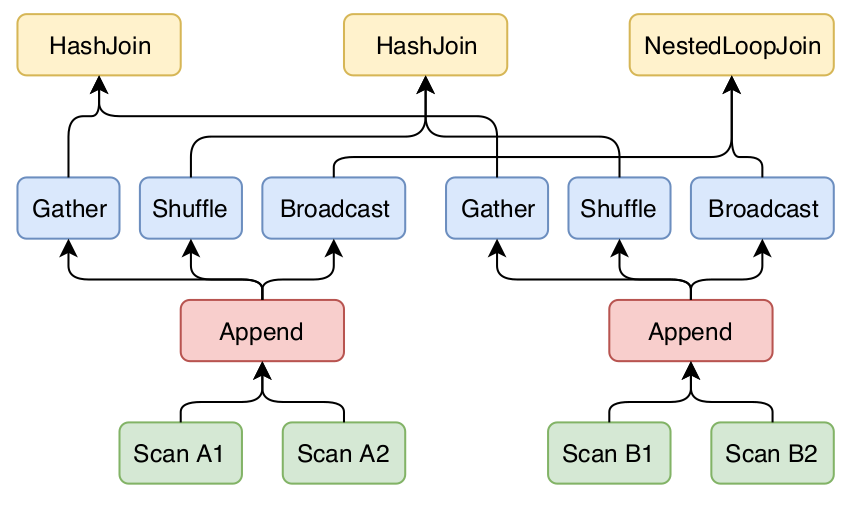
\includegraphics{sharded-plan.png}

\end{frame}

\begin{frame}
\frametitle{Revolución en el ejecutor}

\begin{itemize}
\item El ejecutor estilo ``Volcán'' es ineficiente
\item Para mejorar utilización CPU-caches, paralelismo ...
\begin{itemize}
\item había que rehacerlo con una nueva estructura
\item había que hacer el código más eficiente
\end{itemize}
\end{itemize}

\end{frame}

\begin{frame}
\frametitle{Compilación JIT del ejecutor}

\begin{itemize}
\item Compilación del plan de ejecución a código nativo
\item Actualmente:
\begin{itemize}
\item ``deformado'' de tuplas
\item evaluación de expresiones
\item Mejoras de hasta 30\% en ciertas consultas OLAP-BI
\item ... importante, pero no el fin del mundo
\end{itemize}
\item En el futuro:
\begin{itemize}
\item JITizar los nodos del volcán
\item un cache de programas
\item mejorar generación de código
\end{itemize}
\end{itemize}

\end{frame}

\begin{frame}
\frametitle{Ejecución en ``batch''}

\begin{itemize}
\item Cambiar estilo del ejecutor
\item Permitir que la CPU procese varios registros a la vez
\begin{itemize}
\item  Reduce latencia proporcionalmente a cantidad de trabajo paralelo
\end{itemize}
\item crítico con grandes volúmenes de datos
\item batch + columnar + JIT: 1000x rendimiento (y más)
\end{itemize}

\end{frame}

\begin{frame}
\frametitle{¿Preguntas?}

\centering
¡Gracias por escuchar!
\end{frame}


